% Nama Kelompok : Macintosh
% Kelas : D4 TI 1A
% Anggota : 
% 1. Harun   	1174027
% 2. Fahmi   	1174021
% 3. Kukuh		1174016
% 4. Izzah		1174013
% 5. Rizal		1174014
% 6. Lawimner	1174030




Artikel tentang sejarah Mac OS dari masa ke masa

\section{penjelasan singkat}
Sebelum kita mengetahui lebih dalam lagi tentang MAC OS sebaiknya kita mengenal penciptanya terlebih dahulu
pada zaman dahulu kala hiduplah seorang anak yang bernama \"Steve Jobs\" yang lahir di kota San Fransisco California 
pada tanggal 24 Februari 1955. ia adalah seoarang yatim piatu yang di adopsi oleh Paul dan Clara Jobs.
Berikut perjalanan hidup dan karir Steve Jobs hingga embusan nafas terakhir : 

1955 : di tahun 1955 beliau lahir pada tanggal 24 Februari

1972 : beliau mmelanjutkan pendidikan di perkuliahan tepatnya di Reed College, Portland, Oregon. Tapi ia di drop out setelah semester pertama masuk kuliah

1974 : ia bekerja untuk pembuatan video game Atari dan mengikuti ia juga berkesempatan mengikuti pertemuan Homebrew Computer Club dengan Steve Wozniak, seorang teman sekolahnya yang lebih tua beberapa tahun dengannya. dan Ini merupakan sejenis seminar atau juga bisa di sebut dengan pertemuan yang membahas tema-tema komputer

1975 : Jobs dan Woz kembali menghadiri acara di Homebrew Computer Club Meetings. 

1976 : Komputer Apple tercipta pada April Mob yang jatuh pada tanggal 1 April, tak lama sejak itu jobs dan wozniak membuat sebuah komputer sirkuit baru di garasi Silicon Valley. Pendiri ketiga Apple, Ron Wayne, meninggalkan kerja sama ini, karena setelah hanya dua minggu bekerja. Komputer Apple I dijual pada musim panas seharga US\$ 666,66 atau sekitar Rp.8.658.000 per unit nya

1977 : Apple bergabung dengan beberapa pihak perusahaan untuk membuat kerja sama join venture. Dari situ terciptalah Apple II, komputer pribadi pertama dengan menggunakan grafis berwarna. Pendapatan perusahaan mencapai US\$ 1 juta.

1979 : selanjutnya Jobs mengunjungi Xerox Palo Alto Research Center (PARC). Dari sini ia mendapatkan sebuah ide untuk membuat sebuah komputer dengan graphical user interface yang sangat luas yaitu dapat memfasilitasi tampilan dengan pilihan pada layar berbentuk simbol-simbol 

1980 : Apple kembali mencatatkan sahamnya di bursa saham. Perusahaan mendapatkan dana sebesar US\$ 110 juta. Ini merupakan initial public offering (IPO) terbesar di tahun itu

1982 : adapun Pendapatan per tahun nya perusahaan Apple meningkat hingga mencapai US\$ 1 miliar

1983 : Komputer Apple II dengan menu ikon di layar atau mereka menamakan komputer ini The Lisa diluncurkan ke pasaran dan membuat kehebohan. beliau membujuk John Sculley untuk meninggalkan pekerjaannya di Pepsico Inc. untuk menjadi CEO di perusaan Apple

1984 : untuk meningkatkan daya jual Icon Macintosh di iklankan secara komersial selama acara Super Bowl.dan Macintosh mulai dijual ke pasar

1985 : Jobs dan Sculley terlibat masalah hingga membuat Jobs memutuskan untuk mundur dari perusahaan. seiring masalah itu Wozniak juga ikut mengundurkan diri dari Apple

1986 : Jobs memulai Next Inc. perusahaan pembuatan komputer dengan mesin teknologi yang tercanggih untuk universitas. Dia juga membeli Pixar dari George Lucas, pencipta \"Star Wars\" seharga US\$ 10 juta 

1989 : Komputer First NeXT dijual seharga US\$ 6.500 per unit atau sekitar Rp.84.500.000 

1991 : Apple dan IBM Corp. mengumumkan kerja sama untuk mengembangkan perangkat lunak dan mikroprosesor baru untuk PC. Apple meluncurkan Macs portable bernama PowerBook yang di desain sedemikian rupa

1993 : Apple memperkenalkan Newton, sebuah pena komputer yang bisa digenggam. Perusahaan mencatatkan kerugian hingga US\$ 188 juta pada Juli. Posisi Sculley sebagai CEO Apple digantikan Michale Spindler, yang sebelumnya menduduki posisi Presiden Apple. Perusahaan mengalami restrukturisasi dan Sculley mengundurkan diri sebagai chairman. Selanjutnya, Jobs memutuskan untuk fokus para pembuatan perangkat lunak ketimbang membuat komputer secara keseluruhan

1994 : Apple memperkenalkan komputer Power Macintosh dengan chip PowerPC yang dikembangkan oleh IBM dan Motorola. Apple membuat keputusan agar lisensi perangkat lunak ini dan memberi izin dari perusahaan lain untuk meniru Mac. Adopsi model Mac ini dimenangkan oleh Microsoft Corp. 

1995 : Model adopsi Mac dipasarkan untuk pertama kali. Microsoft meluncurkan Windows 95. Ini menjadikan penggunaan komputer jadi lebih mudah dibanding versi sebelumnya. Apple berjuang terhadap kompetisi dengan perusahaan sejenis, mengalami penurunan di beberapa lini dan melakukan beberapa kesalahan memprediksi kebutuhan pelanggan. Toy Story yaitu sebuah film milik Pixar tiba tiba menggebrak industri layar lebar sebagai film pertama yang menggunakan teknologi animasi. dan kemudian menjadi perusahaan publik di Wall Street dengan mampu meraih dana IPO kurang lebih sebesar US\$ 140 juta. 

1996 : Apple mengumumkan membeli Next senilai US\$ 430 juta untuk pengembangan sistem operasi. Jobs ditunjuk sebagai penasihat di Apple. Gil Amelio menggantikan Spindler sebagai CEO. 

1997 : Jobs menjadi \"interim\" CEO setelah Amelio mengundurkan diri dari perusahaan. Amelio lantas menciptakan produk tandingan bernama iCEO. Jobs pun mengakhiri izin kloning Mac. 

1998 : Apple kembali mencetak untung. Industri komputer kembali dikejutkan dengan produk PC Apple yang diperkaya dengan warna-warna menarik. 

2000 : Apple menghilangkan gelar \"interim\" dan menjadikan Jobs untuk menjadi CEO

2001 : iPod dan komputer dengan operation system X pertama kali dipasarkan. Apple juga meluncurkan perangkat lunak iTunes 

2003 : perusahaan Apple kembali meluncurkan produk nya yaitu iTunes Music Store dengan menjual 200.000 lagu seharga US\$ 99 sen per lagu.dan Ini memberi kesempatan bagi masyarakat untuk membeli musik online secara legal. Lagu di iTunes Store terjual sebanyak 1 juta lagu di awal minggu

2004 : Jobs menjalani operasi akibat penyakit kanker pankreas. Apple mengumumkan penyakitnya setelah Jobs menjalani operasi

2005 : Jobs mengembangkan teknologi iPod dengan menciptakan iPod Nano yang lebih ramping dan iPod yang bisa memutar video. 

2006 : Disney membeli Pixar seharga US\$ 7,4 miliar. Jobs menjadi pemegang saham individual terbesar Disney. Dan sebagian besar kekayaan yang ia raih berasal dari kepemilikan saham ini

2007 : Apple meluncurkan ponsel pintar pertama kali bernama iPhone. Para pecinta Apple rela menginap di depan toko sepanjang malam agar bisa menjadi yang pertama mendapatkan produk terbaru Apple ini 

2008 : Spekulasi penyakit Jobs berkembang hingga spekulasi kematiannya muncul, akibatnya Jobs banyak kehilangan bobot berat badannya

2009 : pada tahun 2009 Jobs menjelaskan perihal penurunan berat badannya karena ketidakseimbangan hormon tetapi dia tetap memimpin Apple. Beberapa hari setelahnya ia mengumumkan untuk sementara meninggalkan Apple guna menjalani perawatan. namun ia kembali bekerja pada bulan Juni. Setelah itu diketahui bahwa ia baru saja menjalankan transplantasi liver

2010 : Apple menjual kurang lebih 15 juta unit gadget barunya, iPad hanya dalam waktu 9 bulan. iPad membuat kategori baru komputer tablet layar sentuh yang lebih modern 

17 Januari 2011 : Jobs kembali mengumumkan akan meninggalkan Apple untuk kedua kalinya karena untuk menjalani perawatan tanpa ada batasan waktu. Cook menggantikan Jobs menjalani operasional di perusahaan

24 Agustus 2011 : Apple mengumumkan pengunduran diri Jobs sebagai CEO. kemudian Tim Cook ingin menggantikan posisi Jobs. Kemudian Jobs menjadi chairman Apple

5 Oktober 2011 : dan akhir nya Jobs menghembuskan nafas terakhirnya di umur 56 tahun. kemudian pada saat itu Apple mengumumkan kematian Jobs tanpa memberikan penjelasan yang spesifik apa yang menyebabkan Jobs Meninggal


\section{sejarah MAC OS}
Macintosh atau di singkat MAC, adalah salah satu jenis berbasis komputer personal berbasis PowerPC yang di produksi oleh apple. Macintosh diperkenalkan pertama kali pada bulan januari 1984 lewat iklan. 
pembuatan Mac merupakan suatu wujud integrasi vertikal yang mana apple memfasilitasi seluruh aspek perangkat keras dan juga sistem operasinya yang terinstall dalam seluruh komputer Mac.

\section{jenis jenis Macintosh}
Nah kemudian ini adalah jenis jenis machintosh atau produk macintosh
Pada tahun 1984 Macintosh mengeluarkan produk pertamanya yaitu Macintosh 128K dan Macintosh 512K.
Kemudian pada tahun 1986 Mac menggeluarkan produk selanjutnya yaitu Macintosh Plus
Pada tahun 1987 mac membuat produk barunya yaitu Macintosh II dan Macintosh SE
Pada tahun 1988 mac membuat Macintosh IIx
Ditahun 1989 mac mebuat cukup banyak produk pada tahun ini yaitu Macintosh SE/30, Macintosh IIcx, Macintosh IIci dan Macintosh Portable
Satu tahhun setelah itu yaitu pada tahun 1990 mac membuat Macintosh IIfx, Macintosh Classic, Macintosh IIsi yaitu seri Macintosh LC
Pada tahun 1991 kemuduian membuat Macintosh Quadra danPowerBook
Ditahun 1992 mac membuat Macintosh IIvx, PowerBook Duo
dan ditahun 1993 membuat 4 produk yang bernama Macintosh Centris, Macintosh Color Classic, Macintosh Performa dan Macintosh TV
Nah pada tahun 1994 mac membuat produk yang awal namanya bukan menggunakan Macintosh ,tapi menggunakan kata power sebagai awal penamaannya yaitu Power Macintosh
Ditahun 1997 juga mac membuat produk baru yaitu Power Macintosh G3, PowerBook G3, Twentieth Anniversary Macintosh
Tapi ditahun 1998 mac hanya membuat 1 produk yaitu iMac
Ditahun berikutnya yaitu tahun 1999 mac membuat 2 produk yaitu iBook, Power Macintosh G4
Pada tahun 2000 produk mac yaitu Power Mac G4 Cube
Dari tahun 2001 mac hanya membuat 1 produk lagi yaitu PowerBook G4
Ditahun 2002 produknya bernama eMac
Ditahun ini pun yaitu pada 2003 mac membuat produk yang bernama Xserve, Power Mac G5, iMac G4
sedangkan pada tahun 2004 juga mac membuat iMac G5
Pada tahun 2005 juga membuat 1 produk yait Mac mini
Dan tahun 2006 membuat produk MacBook, MacBook Pro

	\ref{Gambar1}
	\begin{figure}[ht]
	\centerline{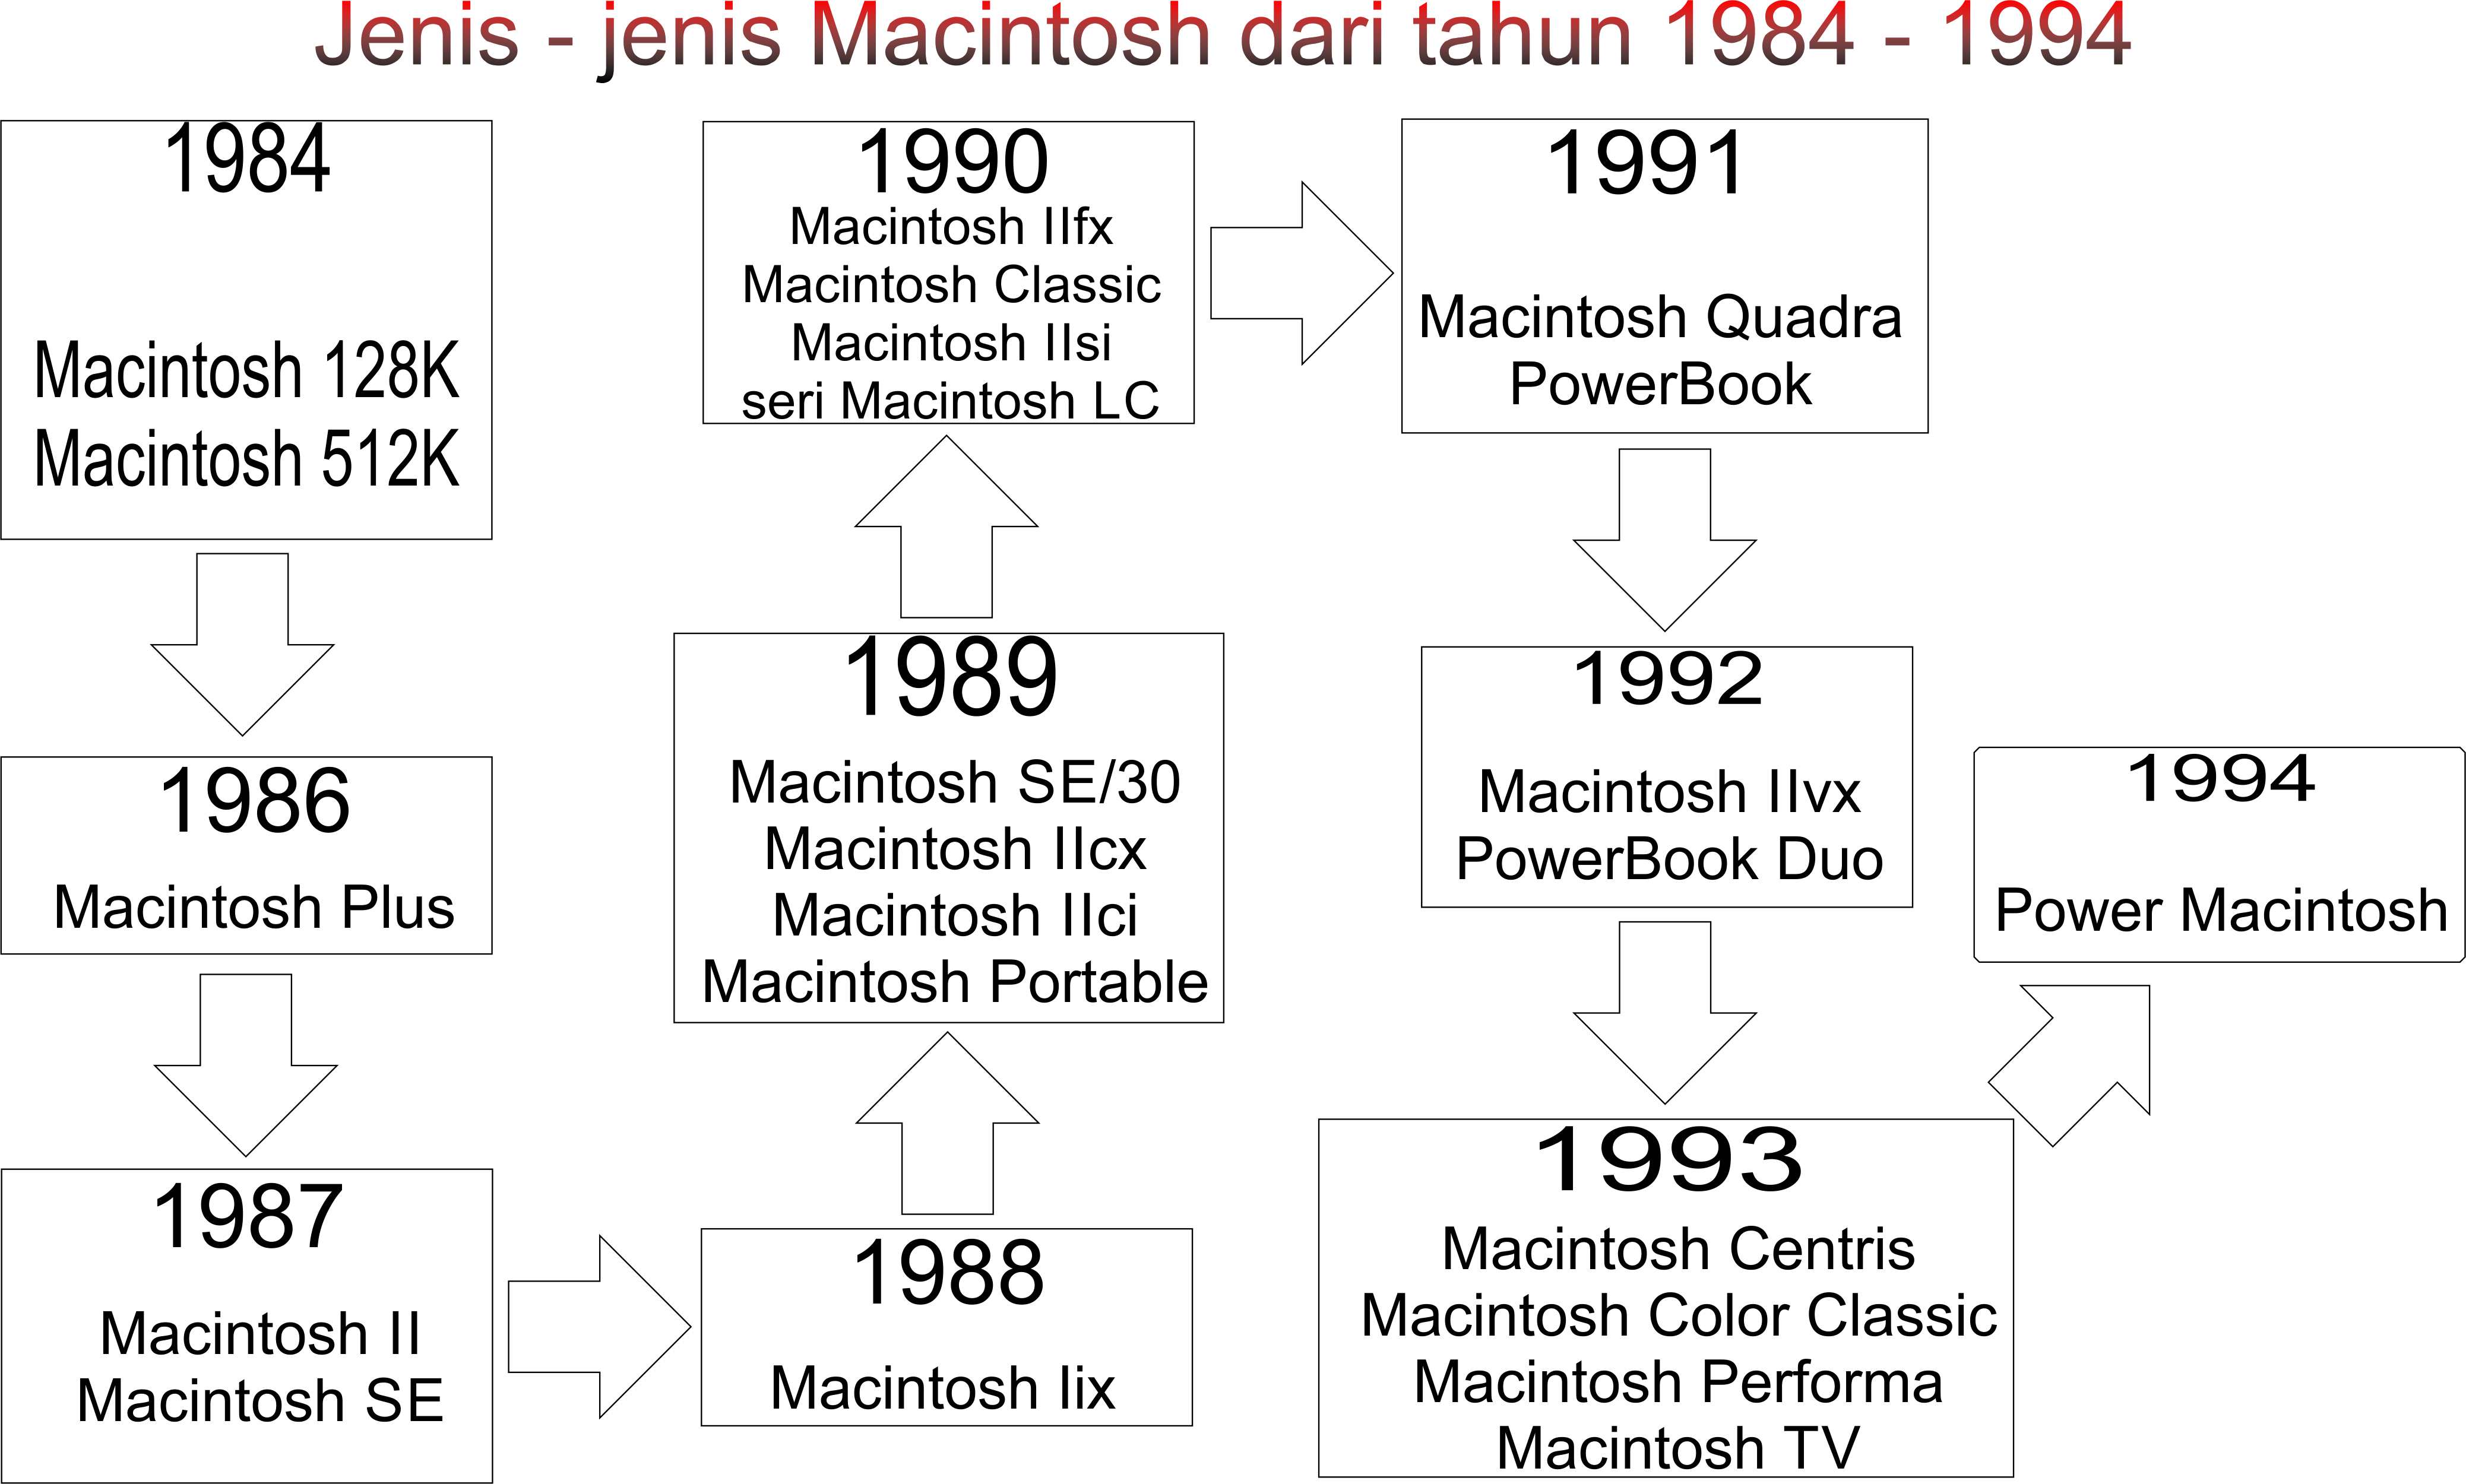
\includegraphics[width=1\textwidth]{figures/Gambar1.JPG}}
	\caption{JenisJenisMacintosh1984-1994.}
	\label{Gambar1}
	\end{figure}

	\ref{Gambar2}
	\begin{figure}[ht]
	\centerline{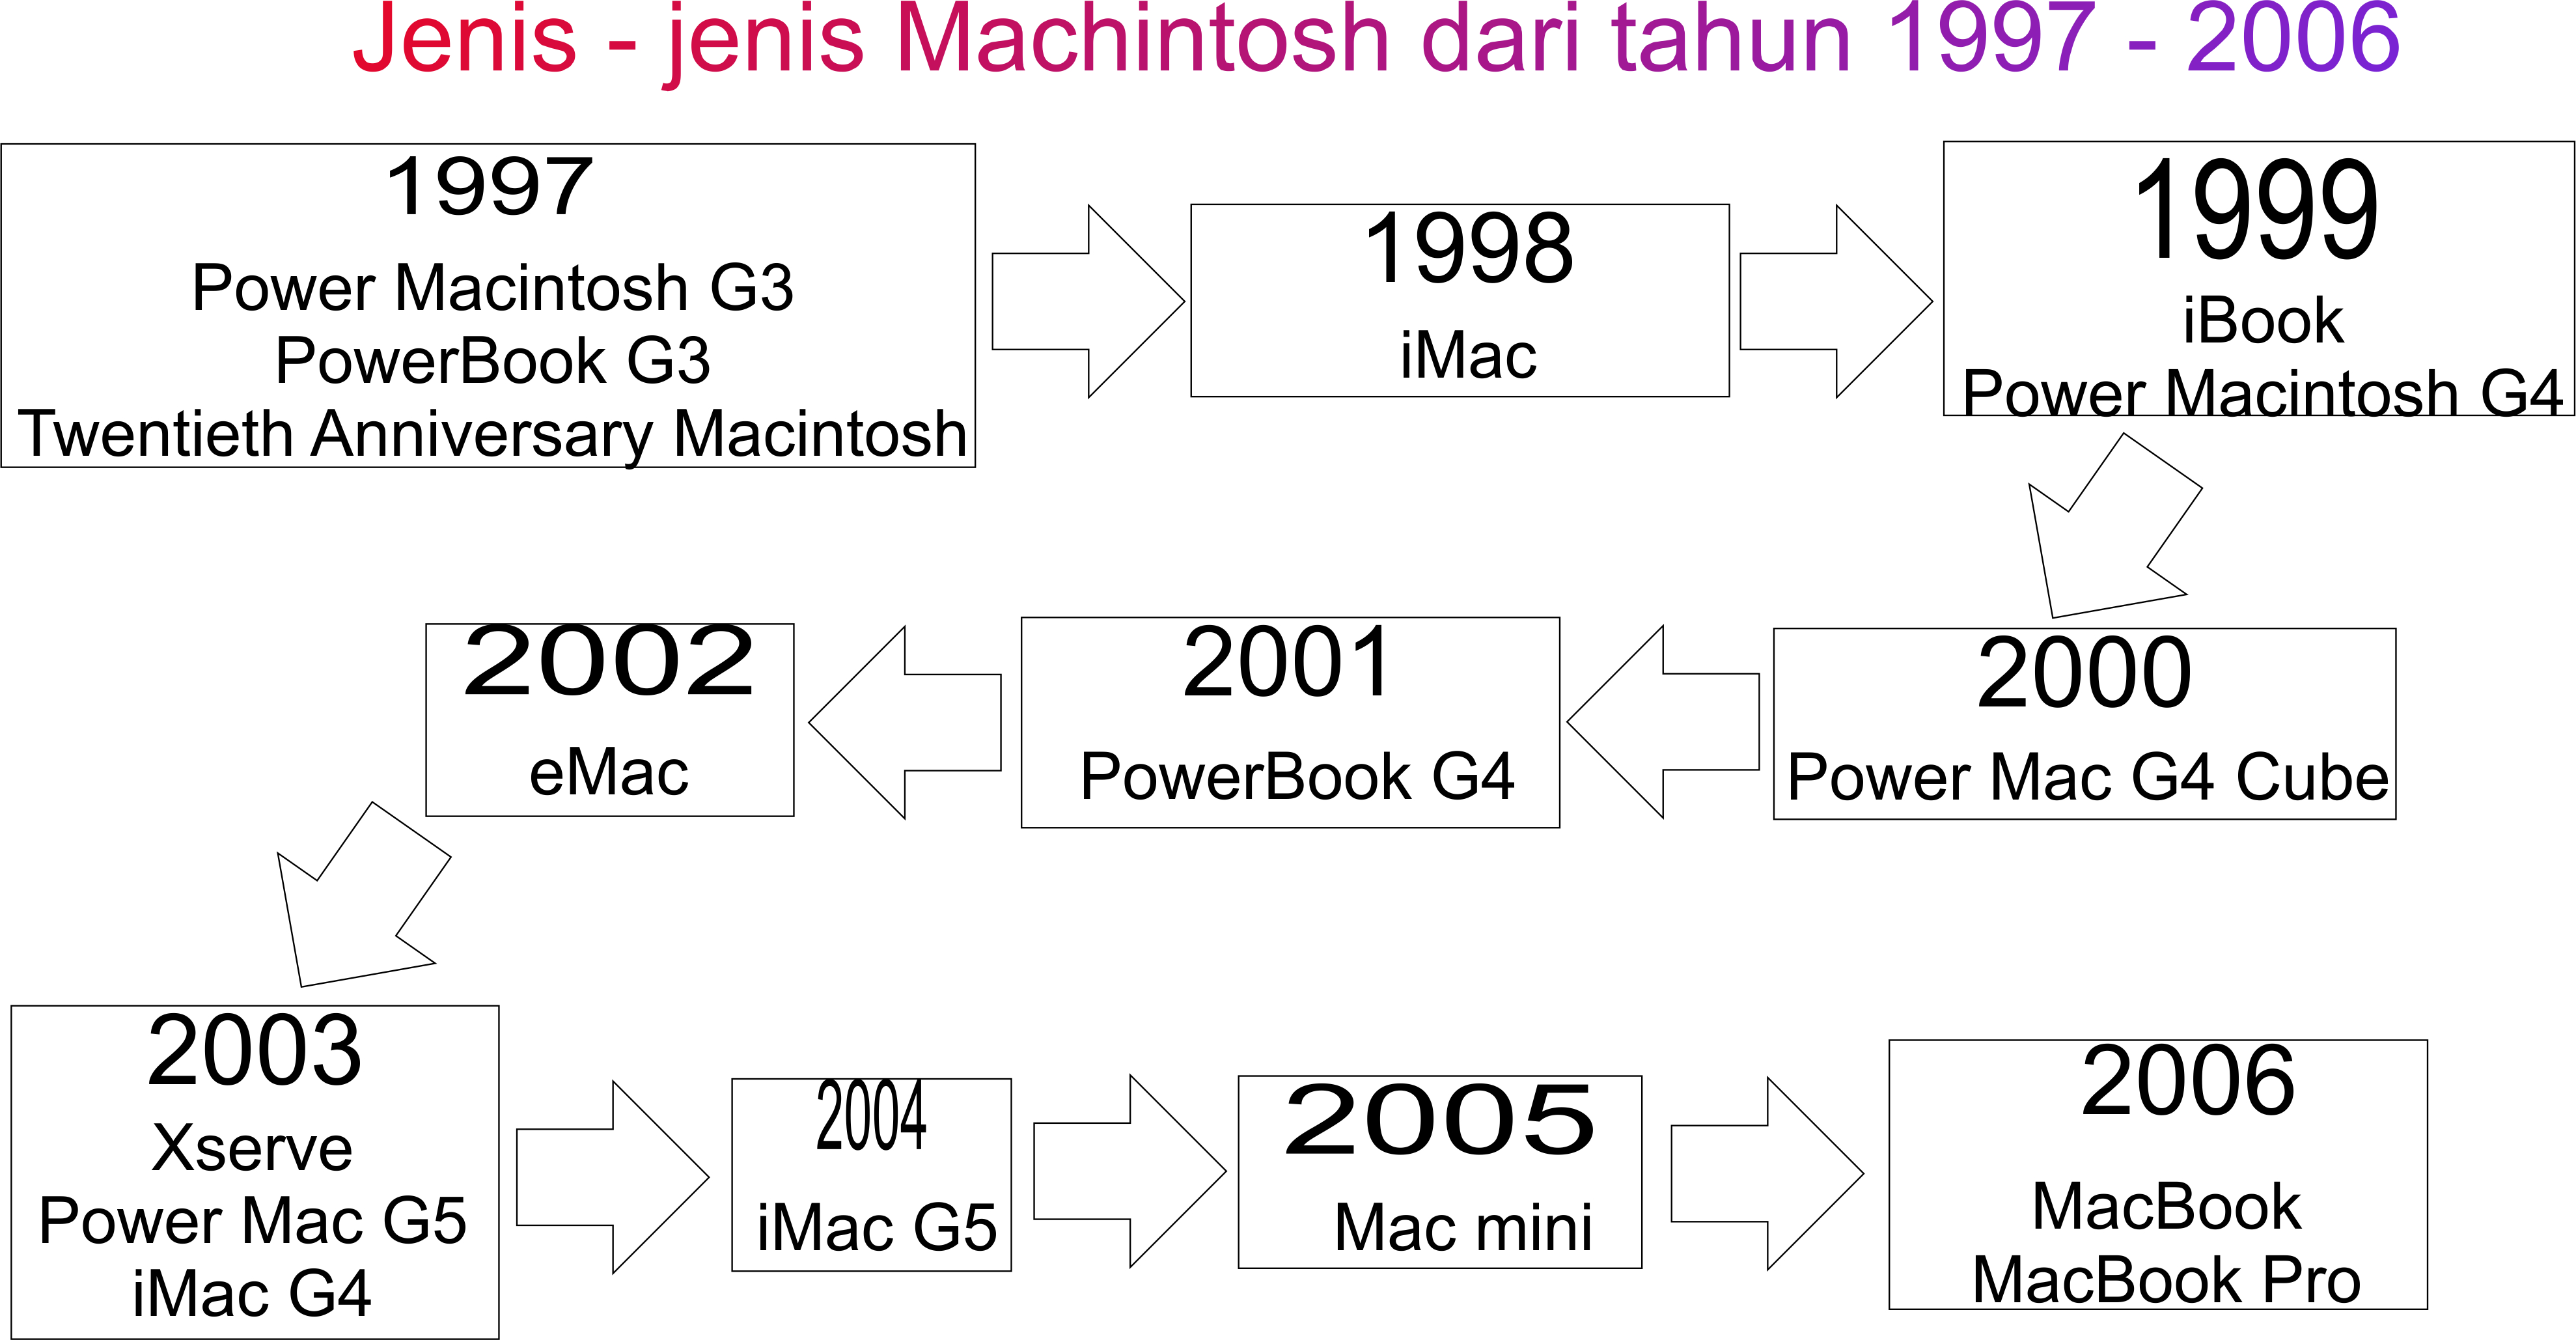
\includegraphics[width=1\textwidth]{figures/Gambar2.JPG}}
	\caption{JenisJenisMacintosh1997-2006.}
	\label{Gambar2}
	\end{figure}

\section{kelebihan dan kekurangan}
Adapun kelebihan dan kekurangan yang dimiliki system operasi Mac OS ini adalah sebagai berikut :

	\subsection{kelebihan}
	-Tampilan yang lebih glossy sehingga bagus untuk desain grafik/multimedia. 
	-Tidak mudah terserang virus, Karena dirancang oleh security oriented. 
	-Machintosh Mempunyai filtur yang bernama “sherlock“ yang fungsinya untuk mencari file pada harddisk dan dalam jaringan lokal, tetapi juga di Internet. 
	-High Performance khususnya untuk MAC OS X yang dapat untuk melakukan semua hal dalam menjalankan aplikasi dengan kecepatan baik. 

	\subsection{kelemahan}
	-Software untuk OS ini belum begitu lengkap seperti pada windows. 
	-Harganya masih terlalu mahal. 
	-Seakan hanya ditujukan untuk desainer grafis. 
	-Kurang cocok untuk aplikasi server dan game. 

Dalam sebuah artikel menyebutkan kekurangan dan kelebihan Mac OS
\cite{linuxwindows}

\section{The Real Leadership Lessons of Steve Jobs}
Enam bulan setelah kematian Jobs, penulis buku biografi terlarisnya mengidentifikasikan praktik yang dapat dicoba oleh setiap CEO.
Steve Jobs mendirikan Apple di garasi orang tuanya pada tahun 1976, digulingkan pada tahun 1985, kembali untuk menyelamatkannya dari kebangkrutan pada tahun 1997, 
dan pada saat dia meninggal, pada bulan Oktober 2011, telah membangun Ini menjadi perusahaan paling berharga di dunia. Sepanjang jalan ia membantu mengubah tujuh industri: 
komputasi personal, film animasi, musik, telepon, komputasi tablet, toko ritel, dan penerbitan digital. Dengan demikian dia termasuk dalam jajaran inovator hebat Amerika, 
bersama Thomas Edison, Henry Ford, dan Walt Disney. Tak satu pun dari orang-orang ini adalah orang suci, tapi lama setelah kepribadian mereka dilupakan, sejarah akan mengingat 
bagaimana mereka menerapkan imajinasi terhadap teknologi dan bisnis. Dalam bulan-bulan sejak biografi Jobs saya keluar, banyak komentator telah mencoba menarik pelajaran manajemen darinya. 
Beberapa dari pembaca itu memiliki wawasan, tapi saya pikir banyak dari mereka (terutama mereka yang tidak memiliki pengalaman kewiraswastaan) tetap mempertahankan sisi kepribadiannya yang kasar. 
Inti dari Jobs, menurut saya, adalah bahwa kepribadiannya adalah bagian integral dari caranya berbisnis. Dia bertindak seolah aturan normal tidak berlaku baginya, dan semangat, intensitas, dan emosionalisme
ekstrim yang ia bawa ke kehidupan sehari-hari adalah hal-hal yang juga dituangkan ke dalam produk yang ia buat. Kelesuan dan ketidaksabarannya merupakan bagian tak terpisahkan dari kesempurnaannya. 
Salah satu terakhir kali saya melihatnya, setelah saya selesai menulis sebagian besar buku ini, saya bertanya lagi tentang kecenderungannya untuk bersikap kasar pada orang lain. \"Lihatlah hasilnya\" 
jawabnya. \"Semua ini adalah orang-orang pintar yang bekerja sama, dan mereka bisa mendapat pekerjaan terbaik di tempat lain jika mereka benar-benar merasa brutal. Tapi mereka tidak melakukannya. 
\"Kemudian dia terdiam beberapa saat dan berkata, dengan sangat sedih\" Dan kami mendapatkan beberapa hal menakjubkan. \"Memang, dia dan Apple memiliki serangkaian hit 
selama belasan tahun terakhir yang lebih besar daripada perusahaan inovatif lainnya di zaman modern: iMac, iPod, iPod nano, Toko iTunes, Toko Apple, MacBook, iPhone, iPad, App Store, 
OS X Lion-tidak untuk
sebutkan setiap film Pixar. Dan saat dia melawan penyakit terakhirnya, Jobs dikelilingi oleh kader rekan yang sangat setia yang telah terinspirasi olehnya selama bertahun-tahun dan istri, 
saudara perempuan, dan empat anak yang sangat mencintai. Jadi saya pikir pelajaran nyata dari Steve Jobs harus diambil dari melihat apa yang sebenarnya dia capai. Saya pernah bertanya 
kepadanya apa pendapatnya tentang ciptaannya yang paling penting, mengira dia akan menjawab iPad atau Macintosh. Sebaliknya dia bilang itu milik Apple perusahaan. Membuat perusahaan 
yang abadi, katanya, jauh lebih sulit dan lebih penting daripada membuat produk hebat. Bagaimana dia melakukannya? Sekolah bisnis akan mempelajari pertanyaan itu satu abad dari sekarang. 
Inilah yang saya anggap kunci suksesnya.
Artikel ini menyebutkan tentang cara kepemimpinan Steve job \cite{isaacson2012real}.

\section{Kesimpulan}
Jadi kesimpulan dari artikel mengenai Macintosh atau MacOS yang telah dapat kita rasakan dari awal kemunculannya pada tahun 1984 hingga saat ini pada tahun 2017 MacOS memiliki 2 jenis yaitu Jenis Mac OS Classic (Klasik) dan Mac OS X sudah Berkembang menjadi banyak Series seperti yg pertama di keluarkannya yaiu System 1, System 2,3,\& 4 hingga yg terakhir dalam MacOS Klasik yaitu MacOS 9 pada tahun 1999. Dan juga dari Mac OS X yang hingga kini dapat kita peroleh dan rasakan mulai dari MacOS X 10.0 dengan nama lain yaitu \"Cheetah\" pada tahun 2001 hingga yang paling terbaru yaitu versi terbaru atau revisian dari Mac OS versi 10.12 yaitu Sierra dengan nama dan serial baru yaitu \"High Sierra\" dengan nomor seri 10.13 yang baru saja rilis pada 2017 ini